As introduced by the background, the project intends to investigate the idea of improving the BSE so that it can produce real financial stock exchange dynamics. To do this, we will be introducing other agents in the financial market, more complex order types and rearrangement of the action-step as well as adapting the new and existing agent parameters so that they can function in the new BSE market. 

\section{Introduction to McG}
McG's paper, as introduced in the background, is focused on introducing realistic market dynamics to Agent Based Models. This project's aim is try to introduce similar dynamics to the BSE by introducing new timing system called ``action steps" and McG agents which claims to produce those dynamics when acting in the same market. The challenge of this project is to adapt the BSE itself in order to implement the agents. 

In the new implementation which this project is trying to achieve is finding a way to integrate these two systems so that the McG agents will be able to mimic the real market environment while retaining the behaviour of ZI-P, ZI-C and Klapan's Sniper so it ensures that the new market implementation is correct. This also includes adapting the McG agent so that it can operate in the BSE market environment. 

\begin{table}[h]
\centering
\begin{tabular}{ |p{4cm}||p{4cm}|p{4cm}|} 
\hline
\textbf{Market Feature}& \textbf{BSE's implementation} & \textbf{McG's requirements} \\
\hline
\hline
Quantity & 1 per order & 1 or more per order \\ 
\hline
Number of unique orders agent can submit if selected & 1 & up to 2\\ 
\hline
Deleting an order & Not fully implemented & Must be implemented \\ 
\hline
Time system & randomly selects one agent per time-step & Ensures that agents have a chance to act in each action-step but not all will act\\ 
\hline
Type of orders & only Limit orders & Limit orders and Market orders \\
\hline
Best price availability & Not always & Must always be available \\
\hline
Price assignments & Agents need to be assigned in order to trade & Agents trade based on only their internal status and algorithm \\
\hline
\end{tabular}
\caption{BSE and McG system differences and changes that must be made}  
\end{table}
\FloatBarrier

As illustrated, a lot of changes in the BSE must first be made to ensure that McG agents can function in the market as well as ensuring that existing agents such as ZI-P, ZI-C and Sniper also maintain their original behaviour.

\section{Introduction to Oesch}
After ensuring that both the new BSE market and McG agents are functioning properly we will test the market with three agents and compare their results to another conference paper by Oesch \cite{Oesch}. McG claims that three of their agents, Market maker, Liquidity consumer and Noise trader, are modelled closely with Oesch's agents. Although Oesch's paper focuses mainly on the price impact function and return statistics analysis, the paper has given example of what is can be expected in terms of mid-price patterns and mid-price return series when three agents (Market maker, Liquidity consumer and Noise agent) are operating in the same market with specific parameters and conditions. This is good benchmark for our agents when they are implemented to ensure that the three agents have functioned properly. 

\section{BSE and McG price assignments}
In the BSE, traders are clearly labeled as either a Buyer or a Seller where they will be submitting only a bid and an ask order in each round. In addition, in the beginning of the trading period, the agents will receive a customer order or ``assignments" notifying them to trade at a specific price and quantity. The agents then can use this information as a factor to make decisions on their orders. Another purpose of the assignment is that they set the equilibrium price of the market and demand-supply curve. 

McG's model does not rely on the assignments like the BSE. It relies on the ``best price" of each side of the book being available in any given time. This is an assumption that matches the real world market since the current spread will always be immediately available if the market is open. 

\begin{figure}[h]
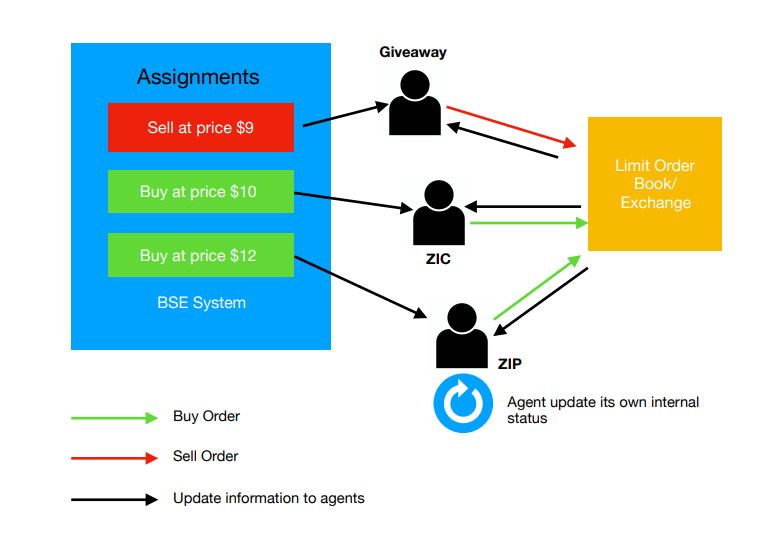
\includegraphics[ height=10cm]{BSE_figure}
\caption{BSE market diagram} 
\end{figure}
\FloatBarrier

\begin{figure}[h]
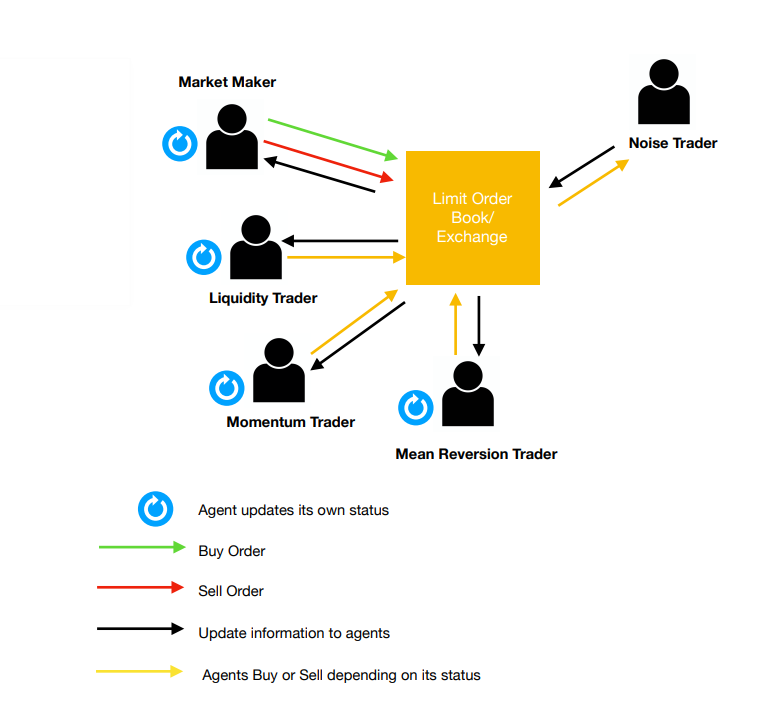
\includegraphics[width=12cm, height=12cm]{McGroarty_figure}
\caption{McG's market model diagram} 
\end{figure} 
\FloatBarrier

\section{Best Price in the BSE}
Some of McG's agents depend on the ``best price" of a side of the book in order to submit an order. This is the highest price in the Bid side of the book and the lowest price in the Ask side of the book. However, unlike the real exchange market, the BSE does not always provide that, more specifically in the beginning of the trading day. This means that there must be some unavoidable modifications to the McG's agents condition regarding order submission. Instead of receiving the best price in each iteration from the LOB directly, the agents themselves will store their own best prices, both ask and bid. These values will be updated each time an order is processed and at the end of each action-step. This mechanism is to ensure that the agent do not run in a situation where the best-price is empty.

\section{Time-step and real market dynamics}
The BSE time-step is easier to understand by giving an example. In a 300 BSE time-step, it is further divided into smaller steps which is equal to the total agents in the market. For example, if there are total of 14 agents in the market, the total number of time-steps in the 300 time period is $300 * 14 = 4200$. In these smaller time-step, an agent is chosen randomly to act in each time-step. 

In their paper, McG suggests that a new system of selecting agents will lead to a more realistic market. Unlike the BSE, the McG ensures that each agent have a chance to act in every action-step. However, this is also dependent on a probability because in the real market, even if the price changes, not trader will be able to follow up and act on it. The probability is implemented based on this assumption. In addition, while BSE agents are required to submit an order if they are selected, the McG agents have two other options of submitting nothing or cancel their order(s). 

However, this leads to a slight problem. By implementing McG style of agent selection without probability of acting,the number of orders in the market will increase which leads to agents such as ZI-P not converging to the equilibrium correctly. This can be solved by introducing the probability of acting for each agent, much like the McG agents. A detailed investigation is presented in Chapter 4 section 4.3. 

\section{Merging assignment based BSE system and McG ``best price" system}
The first change that must be made is that the BSE will give out order assignments to every agent except the McG agents. This will ensure that agents such as ZI-P, ZI-C or Sniper will perform correctly. The ZI-P, ZI-C and Sniper agents will need to be adapted because the selection of agents has now changed. 

\begin{figure}[!htbp]
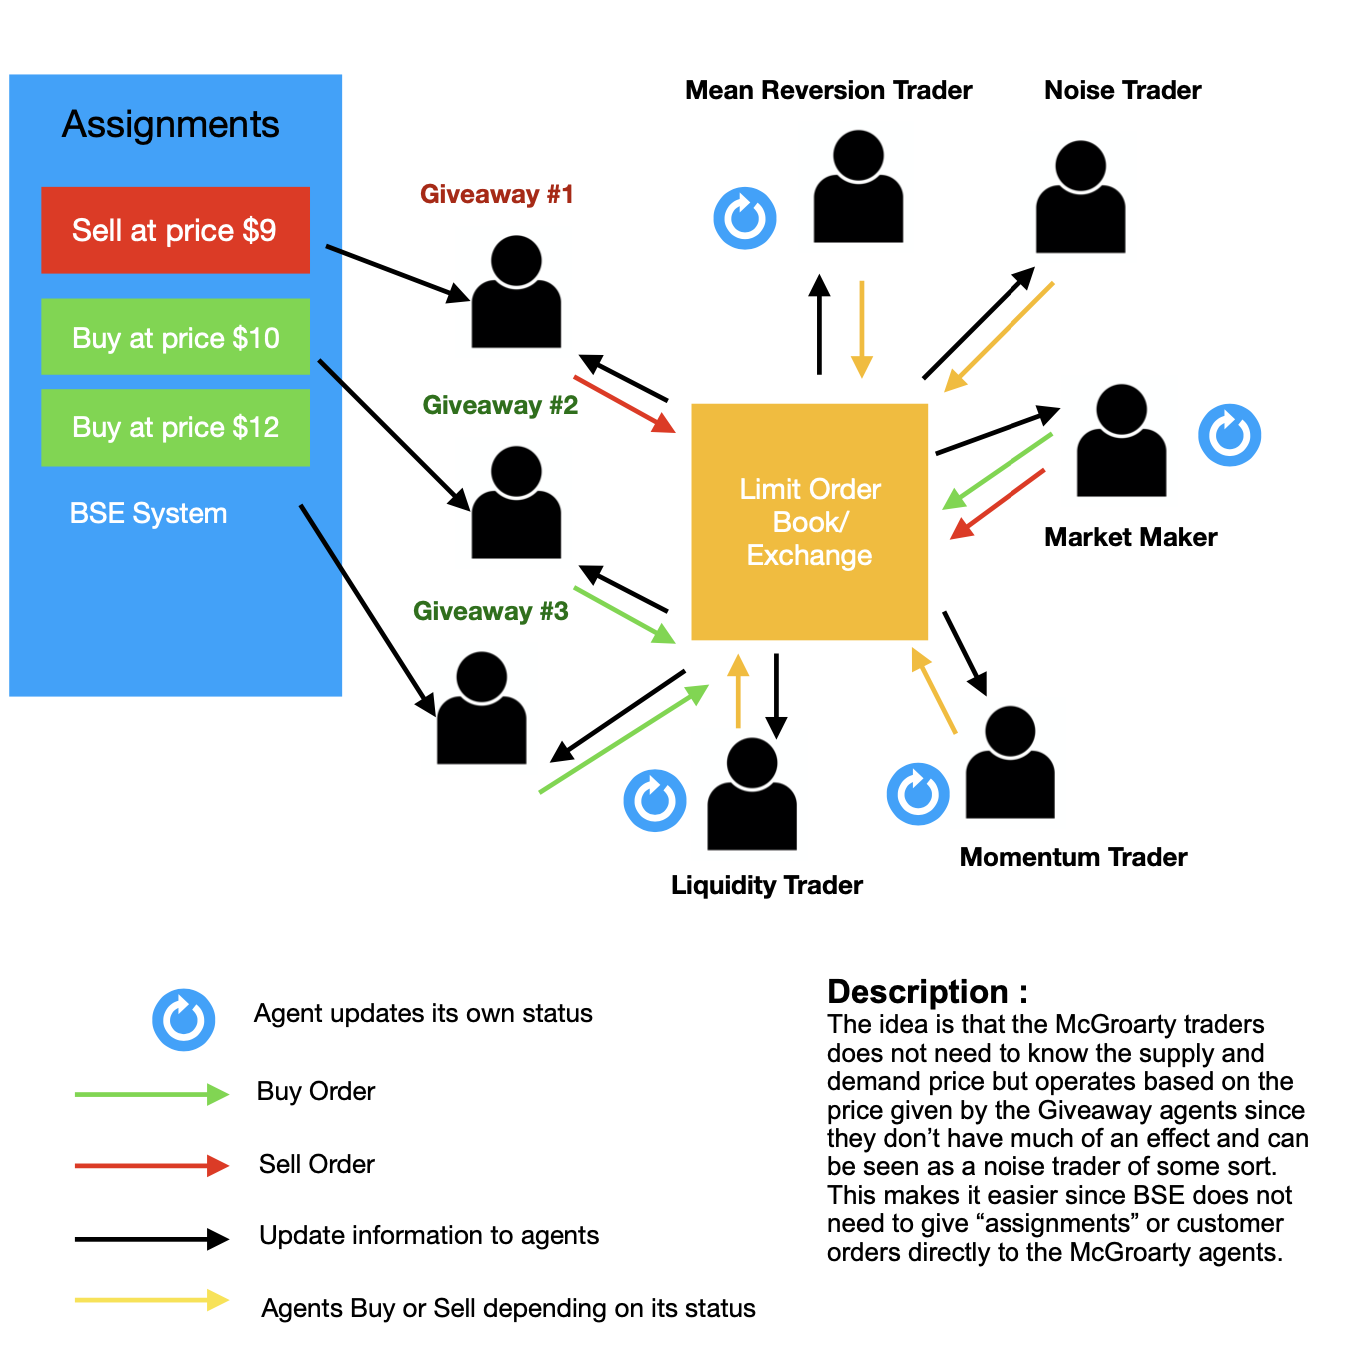
\includegraphics[width=16cm,height=16cm]{Dissertation/images/merge_bse_mcg.png}
\caption{BSE and McG merging market system diagram} 
\end{figure} 
\FloatBarrier

% \end{document} 